\documentclass[11pt]{article}
\usepackage{palatino}
\usepackage[letterpaper,top=1in, bottom=1in, left=1in, right=1in]{geometry}
\usepackage[utf8]{inputenc}
\usepackage{bbding}
\usepackage{amssymb}
\usepackage{graphicx}
\usepackage{setspace} 
\usepackage{rotating}
\usepackage{multirow}
\include{babarsym}
\usepackage[compact]{titlesec}

\pagenumbering{arabic}
%\usepackage{atlasphysics}
\date{}
\newcommand{\tanb}{$\tan \beta$}
\newcommand{\too}{$\rightarrow$}
\newcommand{\rowgroup}[1]{\hspace{-1em}#1}
%\newcommand{\invfb}{$fb^{-1}$}
%\newcommand{\Hp}{$H^{+}$}
%\newcommand{\ttbar}{$t\overline{t}$}
%\title{Multiple Beyond Standard Model Search on the ATLAS Experiment at the Large Hadron Collider}
\title{Search for Beyond Standard Model Phenomena with Tau Leptons and Higgs} 

\author{Haleh Hadavand}

\pagestyle{plain}                     

\textfloatsep  0in

\belowcaptionskip 0in
\abovecaptionskip 0in

\begin{document}
\maketitle
\section{Introduction}
%This proposal describes searches for Beyond Standard Model Physics (BSM) on the ATLAS experiment at the Large Hadron Collider (LHC).  
%This proposal describes Beyond Standard Model Physics (BSM) Higgs searches including exotic Higgs decays that include tau leptons in the final state using the Large Hadron Collider's (LHC) ATLAS Experiment for Run 2 and beyond. 
This proposal describes my research plans in Beyond Standard Model Physics (BSM) Higgs searches at the Large Hadron Collider’s (LHC) ATLAS Experiment, upgrades to the ATLAS detector that I am leading for the high intensity phase of the LHC, 
and plans for integrating my research and education.
LHC's Run 1 culminated in the July 2012 announcement of the discovery of a 125 GeV resonance consistent with Standard Model (SM) Higgs Boson~\cite{atlhi, cmshi}. 
Subsequent measurements of the particle's spin and decay rates indicated that the newly discovered particle was indeed consistent with a SM Higgs~\cite{atlbo,atlsp,cmsf,cmsbo, cmspro}. 

Building on the SM Higgs discovery, the ATLAS Higgs group will be focusing on precision measurements of the SM Higgs properties and searching for BSM phenomena.
%for other Higgs particles.
%The significant increase in center of mass energy and expected data volume for LHC's Run 2 are our best opportunity to discover new physics phenomena in the foreseeable future. 
The increased beam energy and intensity in the LHC’s Run 2 and 3 will likely provide the best 
opportunity to discover BSM physics for at least the next ten years.
The task of discovering it, however, can be more challenging compared to the SM Higgs, whose mass was well constrained by precision electroweak data and the underlying theory, i.e. the SM, 
was well understood and extensively tested for over half a century~\cite{eng,higgs1,higgs2,higgs3}. 
In contrast, the number of theories and models that motivate BSM Higgs searches are significantly larger and more speculative, requiring that a much wider net be cast to cover a broader range of masses and final states. 

One way to look for BSM phenomena is to search for other Higgs particles that are predicted by Supersymmetric theories.  Observing other Higgs particles would mean that the 125 GeV Higgs is part of a more complex Higgs sector.
In this proposal I focus on a charged Higgs search in the $\tau \nu$ final state for early Run 2 data and beyond. As the charged Higgs analysis group convener and being a main analyzer of the $\tau \nu$ final state for Run 1 and early Run 2, I am in an
opportune position to perform this search.  A new endeavor I pioneered will yield the first ever measurement of the intermediate mass region of 160-180 GeV where interference with \ttbar is only recently documented by theorists~\cite{intermediate}.
%We worked with theorists to reconcile interference terms in this region and therefore produce signal samples in this region.  
The intermediate mass region cannot be explored in the H$^+ \rightarrow$ tb final state since there is no way to differentiate the signal from the \ttbar background.

Another way to expand or improve our searches is to use the newly discovered 125 GeV Higgs to bootstrap our way to search for new exotic decays of the Higgs or other BSM states.  
The Higgs mass constraint will help aid the search for signal in a specific region.  %Or one can use the same final states and do a  more global search with no mass constraints by looking for Z+X final states where X $\rightarrow$ ll, including taus.
This method is motivated but not limited to the final states $h\rightarrow ZZ^*$, $A \rightarrow Zh$, $h \rightarrow$ ZZ(dark), $X(h) \rightarrow  Za$, where h is the SM 125 GeV Higgs. 
This proposal combines a search within five theoretical models each decaying to ll$\tau\tau$ and/or $\tau\tau$ll.  With one analysis we are able to
cover all of these models thereby increasing the analysis reach.  The search can be further expanded in a model-independent manner by scanning for Z+X where X can be of masses not theoretically motivated. 
%In this way a search for potential BSM phenomena with no theoretical models can be performed.  



%In Run 1, the BSM Higgs strategy was organized by the motivating models and therefore optimized for the masses, production cross-section, and decay modes of these models. 
%As a result, great efforts were often duplicated where they could have been instead focused on other models, final states, or kinematic regions.  
%The searches outlined in this proposal are organized by final state instead, representing a significant paradigm shift from Run 1. In this approach, interpretation of the results in terms of models is a subsequent step.
%In preparation for High Luminosity LHC which will start detector upgrades in 2023, this proposal describes an upgrade to the detector electronics, namely the Tile hadronic calorimeter low voltage power supplies (LVPS).
%The reliability of the LVPS is crucial to efficient data taking.  There are many challenges which need to be addressed for HL-LHC such as new radiation requirements for the higher luminosity running and as usual tight space and temperature control 
%constraints. I am the L3, or deliverable manager, of this project for the ATLAS detector. This proposal will highlight the methodology for performing research and quality control and producing these components.
In preparation for High Luminosity LHC (HL-LHC), various upgrades of the ATLAS detector to cope with the new conditions are being planned. One of these projects, involving the replacement of the 2048 low voltage power supplies (LVPS) 
required for operation of the ATLAS Tile hadronic calorimeter, became available last year.  
Building on UTA's connections in the TileCal since its inception, I assembled a group and proposed that UTA take over this project. 
Our proposal was well-received, consequently, I am now the L3, or deliverable manager, of this project for the ATLAS detector. The construction phase of this 6-year 
1 million dollar project is expected to be covered by an NSF MREFC proposal in progress. %Project funds are expected to cover the required engineering and materials, but not physicist manpower, 
%so the summer salary provided by this career proposal is critical for me to justify the faith that ATLAS management has shown in me and bring this project to a successful completion. 



%In this proposal, I focus on lepton final states, including $\tau$s.  I propose two different analysis suites which will cover over a dozen final state combinations and about eight BSM channels including a search for charged Higgs.  
This proposal is laid out as follows:
Section 1 covers intellectual merit and broader impact.
Section~\ref{sec:back} gives an overview of my professional background.  
Section~\ref{sec:edu} discusses the integration of research into education.
The motivations for the channels and final states discussed in this proposal are described in section~\ref{sec:mot}.  
Section~\ref{sec:anal} gives an overview of the analysis covered in this proposal.
And finally section~\ref{sec:work} goes over the personnel and the objectives and task list for each analysis.



%The discovery of a charged Higgs would be clear evidence that the 125 GeV Higgs is part of a more complex Higgs sector such as one from the MSSM two Higgs doublet model. It is a much clearer signature than the neutral
%Higgs particles where a further spin analysis would be needed.  I propose to continue my search for charged Higgs in the $\tau \nu$ final state in fully hadronic decays.  This analysis will be important in early data with LHC 
%run 2 since three sigma evidence can be achievable with even a few \invfb of data.  It is also experimentally achievable with a small data with a few to the recently to be published analysis.  
%For this reason this analysis is one placed on the fast track for Run 2 measurements with a goal to present results at Lepton Photon in August of 2015. I propose several ways to increase the background statistics
%and also reduce main systematic uncertainties from this analysis.

%\section{Intellectual Merit}
\input{broaderimpact}


\section{Professional Background}
\label{sec:back}
%Growing up as an immigrant to the United States, the one thing I enjoyed and could control in my life was my studies.  I was always interested in science and 
%wanted to be doctor until I encountered an article in the Scientific American about quantum cryptography.  I became fascinated with the topic and would spend hours
%reading further articles and thinking of ways to fabricate my science fair project which I was hoping to base on that article.  My high school physics program was very limited so I taught myself classical physics and called around to find someone to help
%fund and support my work on my science fair project as it went well beyond my understanding as a high school student.  I finally reached someone working at the Naval Research Laboratory who was excited
%about my project.  Together we built a prototype of an encrypted fiber-optic cable by using a light tight tube and an inner tube for data transmission.  This work sent me to the International Science 
%Fair in Brazil during my junior year in high and started my love for physics.  I knew I wanted to learn about quantum physics and the fundamentals of nature that seemed to defy everything I had learned 
%in my classical physics courses.  

%As an undergrad I worked on a research project within high energy physics tracking electrons in a magnetic field and showed potential in experimental physics.  My junior lab instructor and technician
%mentioned that no other student up to then had performed the experiments individually and successfully in the amount of time it took me to perform them.

\paragraph{Graduate School:}I joined UC San Diego's PhD program since they had a very strong analysis team on the \babar\ experiment slated for measuring $\sin 2 \beta $.  During my first two years while taking courses I traveled to Stanford Linear Accelerator Center (SLAC) to start
learning the basics for performing a high energy physics analysis. My first responsibility as I moved completely over to research was as the Data Acquisitions Manager for the \babar\ detector.  I was on call
for the DAQ system and managed the software repository for Data Acquisition Releases.  I quickly found that a release structure was non-existent, the production area was vulnerable to modifications
and contained untraceable code which would have made it very difficult to recover to the original running state in case of a problem.  I resolved this issue by updating to new production areas once significant code modifications were needed. This greatly improved the reliability and stability of the system.

%I unfortunately missed the $\sin 2 \beta$ measurement by about a year or two and most of the groups talented postdocs vanished to faculty positions. Finding little source of support 

I took an INFN scholarship in Rome Sapienze and in two months produced the best measurement of $\Upsilon(4s)$ to B$^+$/B$^0$ ~\cite{bab0}, a number needed for all B branching fraction measurements. 
%I struggled with a thesis topic and convinced my adviser to perform a time-dependent CP measurement analysis for my thesis.  
%I wanted to perform a time-dependent CP measurement for my thesis topic but during this period it was difficult to find new channels to perform such studies.
My thesis topic was the time-dependent CP measurement of the 3K$^0_s$ final state.
I utilized the vertex IP constraint method allowing for a time-dependent CP measurement although all particles are long lived and therefore do not have a clear production vertex.  
I performed each aspect of the analysis independently from ntuple production to the final limits.  The published paper was the result of my work and another laboratory faculty who performed the branching fraction measurement ~\cite{bab1}.

\paragraph{Postdoc:}I started my postdoc position with Southern Methodist University on the ATLAS experiment.  I was working at CERN at the time and joined the online monitoring software effort. Within a few months I developed a histogram
naming system for the online histograms and modified an existing/decommissioned software for histogram collection to work properly within a new release.  This software was intended for test beam but had never worked properly 
until my modifications.  I also started designing and laying down the foundations for the ATLAS data quality monitoring system.  I was one of the main visionaries, designers, and developers for this system
which is still used both online and offline by ATLAS. My main development contribution was the plug-in algorithms that could be loaded at any point into the system, the online display, and the online time series analysis~\cite{atl5b,atl6}.

During commissioning of cosmics before LHC collisions I setup the entire online monitoring chain from histogram production to final DQ assessments of monitoring data.  This required thorough understanding
of the offline software, within the High Level trigger, and the online environment, software, and tools.  I was the first to develop software to produce $\eta$ vs $\phi$ plots of clusters within the LAr and Tile calorimeters online, use the gatherer to
collect histograms from various monitoring nodes, display the histograms, apply DQ, and time series assessment of the data quality information.  This work gives me a very thorough understanding of the monitoring system on ATLAS both online and offline.

%Before collisions I started analysis on Randall Sundrum(RS) Graviton to diphotons and had the first internally reviewed ATLAS MC results for this final state. From our projections it was clear that with early data we could not make significant measurements in this final state so 
I joined the UED diphoton + Missing Et analysis group for early data taking since the analysis would produce more stringent results with as little as 10 pb$^{-1}$ of data.  With a small analysis team we had one of the first 20 published papers
out of the ATLAS experiment~\cite{atl2}. I was interim editor of this paper and also presented alternative methods of MET calculations for the experiment in addition to being main contributor to the analysis. 

After publishing the UED results I started analysis on Randall Sundrum Gravitons to diphotons where I implemented both a Frequentist tool for setting limits and setup the Bayesian code with BAT for the final limits.  I was
also one the of main analysers in the group.  I was a co-editor for the resulting conference note and paper~\cite{atl1,atl1-conf}.

\paragraph{Research Faculty and Assistant Faculty:}Since I joined UTA in July 2012 I have been working on the charged Higgs to $\tau^+\nu$ in fully hadronic final states.  I have been part of two conference results and two publications ~\cite{hptnu,atl2014,taunu,hptnu1}.
My role on the Run 1 measurement was the high mass background estimation of the $\tau $\too jets background and the statistical treatment leading to the final 
limits for the analysis.  I produced Run 2 projections for this analysis and determined that with only a few \invfb of data evidence of signal can be observed.
I also produced the first intermediate mass samples for the charged Higgs in the mass range of 160-180 GeV.  This was work done with collaboration with theorists to reconcile interference terms in this region. 
For the Run 2 analysis I motivated using the MET trigger instead of the tau+MET trigger used in Run 1.  This choice greatly reduced the trigger and background systematics.  
The background suffered from low statistics when using the tau+MET trigger since the trigger imposed a medium tau selection.  Therefore the matrix method was a comparison
of medium versus tight tau selections where with an MET trigger one could use loose versus tight tau selection hence increasing the statistics.  I also motivated the control region selection
for performing the fake factors method and as a cross check performed a template fit to determine the QCD background~\cite{taunu,hptnu1}.
My work on this charged Higgs final state has resulted in my appointment to the charged Higgs convenership position thereby overseeing all charged Higgs activities on the ATLAS experiment.  

As charged Higgs convener I have motivated new charged Higgs final state searches.  One of these channels is a decay to SUSY final states which would have a signature of three leptons plus missing ET.  Two
of these leptons would be same flavor and opposite sign.  Several independent evidence of an excess in multi-lepton events have been reported on the ATLAS experiment~\cite{3lep}.  I have recently produced MC samples for this final state
using Madgraph and will distribute to analysers to see if the data is consistent with a charged Higgs signal. I have also produced samples for H$^+$\too WZ with final stats of qqll, lvqq, and qqqq.  There are existing analyses that have the same final states as the ones mentioned so a search for charged Higgs signal can be performed fairly quickly.

In April 2016 I was appointed to the position of charge account manager (CAM or L3 manager) for the low voltage power supplies for the Tile calorimeter for HL-LHC.  This account will manage about \$1 million 
of labor, travel, and materials and supplies over a 6 year period.  
%I will oversee the production and testing of half of the  power supplies going into 
%the detector for High-Luminosity LHC.  I am also the deliverables manager for both the LVPS and LVPS boxes which will be assembled by Northern Illinois University.
I have been working closely with Professor Andrew Brandt, the institutional representative for UT Arlington, on this project.
More details about this project are highlighted in section~\ref{sec:lvps} and the schedule is detailed in table~\ref{tab:lvps}.

\section{Integration of Research into Education}
\label{sec:edu}
Since I started teaching in Fall 2012 I have dedicated the first lecture of each class to discuss high energy physics and my research with my undergraduate students who are typically not exposed to this type of information.  I think it is important for them 
to know a bit about our universe and the fundamental questions in physics.  Since the discovery of the Higgs particle the general public has become more aware of high energy physics, but I still see that more than half the students in my
classes do not know about this discovery.  
I have given several colloquium at our university to explain the fundamentals of physics and describe my research to undergraduate and graduate students in the department.  This is a good way to introduce students to our work and
recruit ones interested in high energy physics.  Students typically are very interested in these colloquium and ask lots of questions.  I have also given dedicated colloquium describing the discovery of the Higgs boson.  I explain
the concept of what it means to make a scientific discovery, and show how the signal grew from an evidence to a discovery as we collected more data.  This gives the students a way to relate what they might have heard on the news to seeing the real data and the clear evidence
of the signal.  It is a special experience to be able to show this to students.  I usually go one step further and say that there are potentially other Higgs particles and that I am searching an electrically charged one.
This is something that students typically have not heard about and are excited to imagine there might be other discoveries made in the near future with the LHC data.
This is a great recruiting tool making students excited about being part of a  discovery at the LHC.

This grant, if funded, will support one graduate student, Hussein Akafzade.  Mr. Akafzade has been working with me on charged Higgs searches since the beginning of the LHC Run 2.
I have been teaching him all aspects of doing a physics analysis from production of data samples to setting the final limits.  The learning curve to performing a high energy physics analysis is great.  I am training Mr. Akafzade
to learn ROOT, a statistic analysis package, learning the ATLAS software, extracting data using grid computing, doing analysis to determine QCD background estimates, as well as the statistics and related software needed
to set the the final limits.  Mr. Akafzade will use the experience from the charged Higgs analysis to do this thesis on the Z scan analysis.

The HL-LHC tile LVPS upgrade project will be the thesis topic of Michael Hibbard, an electrical engineering PhD student I have hired to work on this project.  Mr. Hibbard is hired 
through seed funds from the office of Vice President of Research of UTA.  Mr. Hibbard will learn about the physics output of the detector by going to CERN and working on the TileCal test beam.
This project will also hire both EE and physics students to perform the quality control of the LVPS. These students will be trained on using the test stand that has been assembled by Michael and our Electronics Associate Seyedali Moeyadi.


%Since 2013 I have also joined the Long Baseline Neutrino Facility (LBNF) experiment and have been involved in the data quality monitoring of the 35 ton prototype of 10 kton detector.  I have been named the DQ contact and in a short 



%few months have developed a web display to operate as the monitoring and event display for the experiment.  I have also developed a method for others to be able to create monitoring histograms to use with the system.  The current set of monitoring
%histograms used for the TPC volume was developed by myself and a previous UTA research faculty.
%
%For the LHC Run 2 I would like to be involved in the quality assessment of the data.  Run 2 will be a challenging environment with the higher center of mass energy and low mu during initial running.  I have had similar
%experience during the cosmics commissioning period on ATLAS and believe my thorough understanding of the system will be valuable to the experiment.  I have been nominated by several high profile individuals who have served as Data Preparations managers on the experiment to become a Data Quality Convener.  
%The outcome of the search is still pending.
\section{Physics Motivation}
\label{sec:mot}

%The discovery of the Higgs particle in the LHC run 1 and the mapping of the particles properties show that this 125 GeV particle is indeed SM like~\cite{atlsp,cmspro}.  However it is still possible that this particle
%is part of a more complex Higgs sector such as ones predicted by Supersymmetric models~\cite{susy1,susy2}.  %The SM does not explain 95$\%$ of the universe which is predicted to be dark matter. 

%The motivation
%for the LHC energy regime is at the scale to address the hierarchy problem in physics. 
Although the SM has been extremely successful at explaining electroweak data, so-called problems with the theory, such as the quadratic divergence of radiative corrections to the Higgs mass (a.k.a. the Hierarchy problem), and unanswered questions, such as the nature of dark matter, drive our search for new phenomena at the TeV scale. We have strong arguments (i.e. naturalness and the ``dark-matter miracle'') 
that solutions to these problems and questions may be found at this energy. 
The leading theoretical solution is Supersymmetry (SUSY) since it not only addresses the hierarchy problem, but can also provide a dark matter candidate and predicts the unification of gauge couplings at the Grand Unified Theory (GUT) scale.
We also know that the uncertainty of the current Higgs measurements allow for non-SM decays of the Higgs boson of 26\%~\cite{combin} and that theories with SM+singlets have equivalent level of branching fraction~\cite{exohiggs}.

%The five year research plan outlined in this proposal covers several BSM Higgs searches, starting with a broadened version of my Run 1  charged Higgs search in early Run 2. The BSM searches probeSUSY models, for example Next-to-Minimal Supersymmetric Standard Model (NMSSM) that include an additional scalar singlet.  
%The five year research plan outlined in this proposal covers a broadened version of my Run 1 and early Run 2 charged Higgs search as well as a Z+X search in the latter part of the funding period. 

%Table ~\ref{tab:anal} lists all the various exotic Higgs decays, and neutral CP-odd channel.


%Supersymmetry,which is an extension of the SM introduces Supersymmetric partners to the SM fermions, can address both the hierarchy and dark matter problem of the SM.  
%Without the bosons the Higgs
%mass would diverge quadratically and would require fine tuning to keep it consistent with Electroweak measurements.  
%Supersymmetry has been a favored theory because it is able to accommodate these open questions.
%The boson terms which come in as opposite signs in the equation cancel these in the Higgs mass making the 
%fine tuning no longer necessary in most cases.  In R-parity conserving SUSY particles are pair produced and the lightest Supersymmetric particle (LSP) becomes a dark matter candidate. The Minimal Supersymmetric Model and NMSSM where an additional scalar is added to the MSSM both predict 
%more Higgs particles.  In NSSM exotic decays of Higgs such as h \too aa and h \too Z a are also possible.  The NMSSM predicts 7 Higgs bosons while the MSSM predicts 5.  At least one of these bosons is charged another neutral CP odd Higgs is also 
%predicted amongst others. So searches for exotics decays of Higgs and other Higgs particles are well motivated.
  %We therefore know that BSM phenomenon are 
%I will continue the search for charged Higgs in fully hadronic final state of $\tau^+ \nu$ which if discovered would be a clear sign of BSM physics 
%and would imply that the 125 GeV Higgs is part of a more complex Higgs sector. 
%The Charged Higgs is predicted by several models such as ones with Higgs triplets and Two-Higgs-Doublet-Models(2HDM)~\cite{2hdm1,2hdm2,2hdm3}. 
%%The observation of a charged Higgs would be a clear sign of BSM physics and would imply that the 125 GeV Higgs is part of a more complex Higgs sector. 
%In the MSSM, which is a type II 2 Higgs Doublet Model (2HDM), the main decay of charged Higgs at the LHC is t \too b H$^+$ for H$^+$ mass below m$_{top}$. At charged Higgs masses above m$_{top}$
%the main production at the LHC is in association with a top quark.  In the MSSM the Higgs sector can be completely determined by the H$^+$ mass and tan $\beta$, the ratio of vacuum expectation values of the 2HD.
%For masses below the top mass the $\tau \nu$ decay is dominant for $\tan \beta >2 $. In Run 2 we expect that with only a few\invfb of data,
%We will have a much higher chance of seeing this final state due to the larger cross sections (10x in some cases) provided by the higher center of mass energy. The search with 3.2 \invfb of data at $\sqrt s$ = 13 TeV has been recently published ~\cite{taunu}.
%With more luminosity we will be able to probe higher charged Higgs masses so it is important to pursue this analysis up to the entire Run 2 dataset.

Currently the overlap of final states that cross between various physics groups is a point of great discussion within ATLAS management.  The optimization of analysis and the ability to perform 
cross checks within similar analyses is important for the race to find new physics in Run 2.  With the new ATLAS data model based on xAODs and no longer depending on group specific Derived Physics Data we can start to achieve that goal.

We, however, have to go one step further and think of making an analysis suite that can be simply ported for several analyses with similar final states by simply leaving some selections as variables to 
be tweaked.  This will save time since people are not duplicating writing selection code, applying combined physics group systematics,  and again allows for simple cross checks across groups.  

With those requirements in mind I propose a single analysis suite where we can perform the Z+X search which is motivated by several channels listed in table ~\ref{tab:anal}.
The Z+X search will primarily probe SUSY models for example Next-to-Minimal Supersymmetric Standard Model (NMSSM) that include an additional scalar singlet or SM +singlet models.  It can also be used to discover other states not theoretically motivated therefore investigating new mass regions where potential new particles could exist.
%Additionally I propose searching for final states in the range $12<$ m$<60$ where a``dark'' Z that serves as the mediator from a new U(1) gauge symmetry that can serve as the portal to a hidden sector that constitutes dark matter~\cite{zdark}. 
Additionally I propose searching for a ``dark'' Z in the mass range $12<$ m$<60$. A ``dark'' Z serves as the mediator of a new U(1) gauge symmetry that can serve as the portal to a hidden sector that constitutes dark matter~\cite{zdark}. 
Notice that in total there are five different theoretical models that decay into two different final states.  This is a great triumph over analyses that would at most cover a few final states.
Table ~\ref{tab:anal} summarizes all the channels and final states covered in the Z scan analysis.  Notice that each channel has the 125 GeV Higgs either in the initial or final state. 
Using the newly discovered Higgs particle in a broad scan will expand the experimental reach of this search.
%The second analysis suite is an extension of the \Hp to $\tau\nu$ search to include an additional $\tau$ opening the bb$\tau\tau$ final state.

\begin{table}[h]
\begin{center}
\begin{tabular}{ l |  l    |  l                   | l         || l    }  \hline 
 Analysis   & Channels        $\rightarrow$  &  $\tau \tau$ ll  & ll $\tau \tau$  &   Theory  \\ \hline \hline
\multirow{4}{*}{Z Scan} & $h\rightarrow ZZ^*$ &  $\checkmark$ & $\checkmark$                     & SM \\  

  &$A \rightarrow Zh$            &                    & $\checkmark$     &   MSSM, NMSSM \\  
  &$h \rightarrow$ ZZ(dark)  &    $ \checkmark$          & $\checkmark$  &dark U(1) gauge     \\   
  &$X(h) \rightarrow  Za$ for a l=$\mu$  &  $\checkmark$      & $\checkmark$ &   NSSM, SM+singlet\\ \hline \hline
%\multirow{2}{*}{$\mu$ Scan} & $h \rightarrow a a$  $l=\mu$ &    \checkmark            &\multicolumn{2}{c||}{$\checkmark$} & NSSM, SM+singlet\\
%  &$h \rightarrow$ Z(dark)Z(dark) & \checkmark &\multicolumn{2}{c||}{$\checkmark$}             & dark U(1) gauge\\\hline 
% & $H(G) \rightarrow hh$  & \multicolumn{3}{c||}{}  &   extra-dimensions , 2HDM\\  \hline

    \hline
    \end{tabular}
    \caption{ Table showing channels and accessible final states and theoretical models for several BSM models including the standard model h \too ZZ$^*$ channel~\cite{hexotic}.  The mass of the scalar singlet a and Z(dark) are  $4  <m(a)< 10 $GeV   $15 < m(Z(dark)) < 60 $GeV respectively.}
\label{tab:anal}
\end{center}
\end{table}
My strategy is to combine several final states and channels to increase statistics and look for a bump using a bump-hunting procedure I developed as a first pass. The approach removes the need for setting limits in a fine granularity in the discriminating variable, thereby greatly speeding up the statistical analysis. This speedup will allow for quicker turn around of searches in the absence of signal.  In the end the full statistical treatment as recommended for ATLAS will be performed to present the final results but this first pass will allow for flexibility in the search. 

%This initial statistical assessment of the data will allow the analyzer to promptly respond to any potential observed excess.  This procedure can be used even for a 'blind' analysis where the signal area is hidden to prevent analyzer bias.  The result will be a quicker and broader search without wasting time on focusing on areas devoid of BSM signal.  This iterative statistical treatment procedure will save time and effort which can be spent on new BSM searches.

While we hope to find BSM at the TeV scale, we have not seen any smoking gun evidence thus far.  It is preferential to search as broadly as possible for BSM.  Thus far the searches for other Higgs particles and exotic Higgs decays have been very model specific and based on analysis optimized for a specific theory.  A broad search with no mass or model assumption is more likely to observe something new, allowing us to efficiently look for several models simultaneously.  If evidence for signal is found in this broad and quick search,  a subsequent targeted and optimized search can be performed, taking into account any potential bias from the first step.


%Our current results exclude the existence of a charged Higgs below 150 GeV in the high mass however we are not yet quite sensitive enough 
%since above the top mass the tb final state is dominant. The intermediate region of 160-200 GeV has not been treated due to the fact of not being to reconcile interference effects. There are however LO calculations and NLO calculations to be made available within the time scale of Run 2.
%It is however possible to get LO  predictions using MG5\_amc and then scale the total cross section to NLO t$\overline{t}$.  

%The addition of this mass region will close the gap mH vs \tanb mass range and also produce competitive results at low \tanb vs A \too $\tau \tau$ and \Hp \too t$^+$b.  With 13 TeV projection we see that with only a few $fb^{-1}$ of data  we can have evidence of the particle if it exists.   
%Run II will have a much higher chance of seeing this final state given that cross sections with the higher center of mass energy will increase up to a factor of 10 in some cases.
%This analysis is one placed on the fast track for Run 2 measurements with a goal to present results at Lepton Photon in August of 2015.  
%%By using simulated t$\overline{t}$. instead of $\tau$ embedding this should be achieved with early data.  The jet to tau background statistics can also be improved hence reducing one of the main systematics in the current analysis.  

%Extending the charged Higgs analysis suite to include an additional $\tau$ should be a trivial task.  The low mass charged Higgs search already requires a b jet and a $\tau$.  A high mass search requires the addition of b jet coming from the associated top.
%The addition of  another $\tau$ to the final state is a natural extension of the existing analysis, allowing observing new final states h \too a a, Graviton \too h h , and H \too h h with  h \too bb $\tau \tau$.  This covers both MSSM, NMSSM theories and extra-dimensional theories including Gravitons.  

%My strategy is to combine several final states and channels to increase statistics and look for a bump using a proprietary bump-hunting software which will speed up traditional limit setting procedure.  Of course the standard ATLAS methodology for setting limits
%should be adopted in the end but this intermediate statistical treatment will allow for quick searches with early Run 2 data.  Again we want to look everywhere but we do not want to take forever doing so, so we need to move on from areas where we know
%new physics cannot exist and be flexible in our searches. So the analysis will have several passes of analysis one starting to be quite general then and can successively become more detailed.

%The H$^+ \tau^+ \nu$ analysis is well motivated by Supersymmetric models such as  the Minimal Super Symmetric Model (MSSM) for having the largest BR at low mass and the second highest BR after the tb final state in higher
%\tanb and higher masses.   
%In the intermediate region of 160-200 GeV the $\tau \nu$ BR dominates.  This fact is important for Run2 measurements where we can start to look into
%the intermediate region with early data and potentially exclude the low \tanb region and can potentially outperform the H$^+$ \too $\tau \tau$ final state in this parameter space. 


%EXTRAS:
%Our studies also show that with only a few fb$^{-1}$ of data we can supersede the Run 1 results based on 20 fb$^-1$ at a center of
%mass energy of 8 TeV.  In MSSM \tanb vs mH plane this final state has the potential of outperforming the H$^+$ \too $\tau \tau$ final state by closing the gap at low \tanb. It is for these reasons that the H$^+ \tau \nu$ final state will be one the first results with the LHC run 2 and it is of high priority.
%
%The $H^+ $\too $\tau \nu$ final state searches have already restricted the existence of the charged Higgs at masses lower than 150 GeV with the benchmark MSSM mhmax+ model. 
%I propose to add the intermediate mass region of 160-200 GeV which was previously left out since no theoretical predictions of the top interference in this region was known.   It is however possible to get LO 
%predictions using MG5\_amc and then scale the total cross section to NLO t$\overlin{t}$.  The addition of this mass region will close the gap mH vs \tanb mass range and also produce competitive results at low \tanb
%vs A \too $\tau \tau$ and \Hp \too t$^+$b.  With 13 TeV projection we see that with only a few $fb^{-1}$ of data  we can have evidence of the particle if it exists.   
%Run II will have a much higher change of seeing this final state given that cross sections with the higher center of mass energy will increase up to a factor of 10 in some cases.
%This analysis is one placed on the fast track for Run 2 measurements with a goal to present results at Lepton Photon in August of 2015.  By using simulated t$\overling{t}$. instead of $\tau$ embedding this should be achievable 
%with early data.  The jet to tau background statistics can also be improved hence reducing one of the main systematics in the current analysis.  

 
\section{Research Plan}
\label{sec:anal}
The analyses discussed in this proposal are \Hp to $\tau^+ \nu$ and Z scan with Higgs and taus.  The charged Higgs analysis will be the focus of my research plan for the first two years and will continue as we reach 
higher luminosities.  In the second year I will start a new endeavor in the Z scan analysis.  I will use my experience with taus to look for final states with this particle.  
%1. and 2. would be part of the same analysis suite since they have very similar final states. By adding and additional
%tau to the charged Higgs analysis one gets 3.  
%2. and 3. are part of one analysis suite since they have leptons and taus in the final states.  With slight additional requirements on a basic set of ntuples one can get either the Z or muon scan.
In the sections to come I will give an overview of each analysis and in the workplan in section~\ref{sec:work} go over specific objectives and tasks for each analysis.

In addition to these two analyses there is an upgrade component for HL-LHC.  The details of the project are included in section ~\ref{sec:lvps}. Table~\ref{tab:lvps} highlights major milestones of the project.

\subsection{Charged Higgs Search in the $\tau \nu $ Final State}
%The Charged Higgs is predicted by several models such as ones with Higgs triplets and Two-Higgs-Doublet-Models(2HDM). The observation of a charged Higgs would be a clear sign of BSM physics and would imply that the 125 GeV
%Higgs is part of a more complex Higgs sector. In the MSSM, which is a type II 2HDM, the main decay of charged Higgs at the LHC is t \too b H$^+$ for H$^+$ mass below m$_{top}$. At charged Higgs masses above m${_top}$
%the main production at the LHC is in association with a top quark.  In the MSSM the Higgs sector can be completely determined by the H+ mass and tan $\beta$, the vacuum expectation values of the 2HD.
%For masses below the top mass the $\tau \nu$ decay is dominant for $\tan \beta >2 $. Our current results exclude the existence of a charged Higgs below 150 GeV in the high mass however we are not yet quite sensitive enough 
%since above the top mass the tb final state is dominant. The intermediate region of 160-200 GeV has not been treated due to the fact of not being to reconcile interference effects. In recent discussions with theorist
%it has been determined that a LO calculationon can be achieved easily using MG5\_amc5 and that NLO calculations should come before the LHC run2. 
%
%I propose to start looking at the LO samples to determine luminosity projections for run 2 since the tau nu channel can be more sensitive than the A \too $tau tau$ final state at low tan $\beta$ in this mass range.
%It is however possible to get LO  predictions using MG5\_amc and then scale the total cross section to NLO t$\overline{t}$.  
%Run II will have a much higher chance of seeing this final state given that cross sections with the higher center of mass energy will increase up to a factor of 10 in some cases.
%This analysis is one placed on the fast track for Run 2 measurements with a goal to present results at Lepton Photon in August of 2015.  
The charged Higgs analysis is a direct search for a Higgs triplet or 2HDM.  Our current results exclude the existence of a charged Higgs below 150 GeV in the MSSM mhmax scenario. In the high mass however we are not yet quite sensitive enough 
since above the top mass the \Hp \too t$^+$ b final state is dominant~\cite{hptnu}. 
The intermediate region of 160-180 GeV will be performed by the end of the year.  Only recently have theorists been able to reconcile \ttbar interference effects supply us with NLO  calculations of the cross section as a function of mass and \tanb.
The addition of this mass region will close the gap mH vs \tanb\ mass range and also produce competitive results at low \tanb\ vs A \too $\tau \tau$ and \Hp \too t$^+$b, see Figure~\ref{fig:brlimits}.  With 13 TeV projections we observe that with only a few $fb^{-1}$ of data we can have evidence of the particle if it exists.
By using simulated \ttbar data instead of $\tau$ embedding this analysis was able to publish results with 3.2 \invfb of 13 TeV data. The jet to tau background statistics for the Run 2 analysis were much better than Run 1
by using my suggestion of only using a missing ET trigger as opposed to a tau plus missing ET trigger.  The use of the tau in the trigger implied that a medium selection of taus had to be used in the fake factor method, where in Run 2 we could use a Loose selection therefore greatly enhancing the statistics.

%% HH fix analysis cuts
\subsubsection{Selection and Backgrounds to \Hp $\tau\nu$}
The selection for the \Hp analysis include the following 1.  ETmiss trigger, 2. $\tau$ with pT $> 40 $GeV, 3. At least 3 jets for heavy \Hp with pt $> 25$ GeV, 4. no electron or muon,
5. ETmiss$ > 150(TBD)$ GeV for heavy(light) \Hp, 6.  at least 1(2) b tagged jet light(heavy).  The final discriminating variable used is 
$m_T = \sqrt{ 2p^\tau_TE^{miss}_T(1-\cos {\Delta \phi_{\tau_{had-vis},miss}})}  $

There are three major sources of background to the \Hp analysis.  They include 1. true $\tau$ background 2. QCD background 3. leptons faking $\tau$s.  1. and 2. were data driven for Run 1 while 3. is taken from MC simulations.  
For the early Run 2 analysis only the QCD background was taken from data.  The other two backgrounds were derived from MC simulations. As a crosscheck, for the ICHEP 2016 results the shape of \ttbar\, true $\tau$ background was taken
from MC while the normalization was taken from the fit to data.

%\subsubsection{bb $\tau \tau$} 
%The bb $\tau \tau$ final state is achievable with an additional $\tau$ added to the high mass charged Higgs analysis.  This is a final state coming from the decay of h\too a a \too bb $\tau\tau$ which can describe the Fermi-Lat data that shows evidence of gamma ray excess in the galactic center of the universe.
%One can also have a Graviton or a higher mass CP even Higgs, motivated by SUSY, decaying to this final state.  For Run 2 one of the challenges will be the trigger one can use.  With the additional $\tau$ the trigger would be different than that of the charged Higgs.  In order to combine
%the analysis suite successfully this issue has to be reconciled.  This channel has different challenges whether the intermediate particle is reconstructed as a Higgs or a scalar singlet a.  The low mass singlet channel will have low pT objects which can be difficult to reconstruct.  It is for this reason this analysis is one in which I would potentially get involved if another student and therefore
%additional manpower would be available.

\subsection{Z+X including Higgs and taus}


%Table ~\ref{tab:anal} shows how we can combine two analysis suites to essentially do three analysis covering all the channels.  
%Many of the channels in table 1 have a Z boson in the final state.
%One analysis for the multiple BSM search includes a scan of particles associated with a Z in the final state (top left portion of table).  
%Another will be a scan of dimuon events (bottom left portion of table). %And the final will be an extension of our charged Higgs
%analysis where we only need to add a tau lepton to the high mass analysis for the charged Higgs. The X in the table shows final states which are not covered in this proposal. 


For the Z mass scan I propose to perform two mass scans constraining the given particle combination to the Z mass and scanning in the 'other' particle. 
For example, Z(ll) other($\tau\tau$) and Z($\tau\tau$)other(ll) would be two separate scans of the 'other' particle after requiring that the event has a Z particle. 
The mass range of the scan would go from 4 GeV to 2 TeV and each object would be a resonance in that mass spectrum. The ee and $\mu\mu$ channels are added together 
in one spectrum since they have similar resolution and hence can increase the statistics for bump-hunting.  
The two scans, one with taus and the other with l=$\mu$,e  can then be combined together with a statistics framework.  

%leptons, reconstruct the mass and look in a range of 30 GeV to 2 TeV.  Similarly one can see from the channels in columns 3 and 4 (before the double lines) of the table that the same logic of scanning for the 'other particle' can be done over the same 
%region in mass. It is important to be able to combine the various physics models in one analysis since there are gaps in mass in the searches in the current Run 1 analysis.  These gaps need to be explored in our search for BSM
%phenomemon in Run 2 to make for a complete search.  
Of course the 4 lepton final state is one that is extensively tested for the SM ZZ* final state. This analysis would add the ll$\tau\tau$, $\tau\tau$ll final states to this channel for the first time.  The resolution will not be as favorable as
the 4 lepton final state but by constraining the on shell Z to decay to $\tau \tau$ one can improve the mass resolution.  These final states can add further sensitivity to this channel specially as the LHC
gathers more data.  With about 10 \invfb\ of data at the center of mass energy $\sqrt s$ = 13 TeV the 4 lepton analysis observed 3 events per category including a combination of electrons and muons.  The efficiency for tau reconstruction is lower (30-40\% as opposed to around 80\%) than the electron and muon channels and in 
addition pose a more challenging final state due to the existence of neutrinos.
However on average $35/80\times4\sim 2$ ($2\tau2e, 2\tau2\mu, 2e2\tau,2\mu2\tau$) events/10\invfb can be added to this channel~\cite{2016:4l} increasing the total statistics by 2/12=17\%. With a final dataset of 250\invfb of data this would be a significant addition to the existing channels.

%In the case that the sensitivity is not improved with this final state, this channel could be important for studying the missing ET in the diboson final states of the Higgs.
%It is entirely possible however that this final state will not improve the sensitivity in this channel but 
%In Run 1 several SM Higgs events had large associated missing ET and in one case a 4$\mu$ final state had MET of$\sim$ 100 GeV.  It would be interesting to see if more high MET events can be seen with the addition of the ll $\tau\tau$ statistics to this channel.

%A muon scan would be used to look for the channels h \too a a and Z(dark) Z(dark) final states. The lower predicated masses for these particles, $4  <m(a)< 10 GeV$  
%$15 < m(Z(dark)) < 60 GeV$, makes it natural to combine these two scans.  Granted that for h \too aa the $\mu\mu \tau \tau$ final state has the largest branching fraction and for the h \too Z(dark) Z(dark) the 4l final state has the 
%has the best resolution but in doing one analysis is it trivial to add the other final state and therefore increase statistics.  I would also not restrict this analysis to the mass range predicted for the a and Z(dark) particles but extend to masses of order 1 TeV.


%In building the analysis suite for \Hp $\tau \nu$ final state for high mass one needs to require at least two b jets and one tau in the final state.  At this point one can write out ntuples for the analysis and also allow for
%the option of adding an additional $\tau$ object to the final state. In this way one can have the $\tau\tau bb$ final state that can come from h \too aa or G(H)\too hh  within  the same framework. 
%I am sure there are many more overlaps that I am not covering in this proposal but this idea is presented here to make the point that overall discussions amongst physics groups are important before Run 2. People do no want to repeat the data redundancy and computing inefficiencies that happened during Run1.  Now it the time to take some action to prevent this for Run 2 by better organizing our analysis.  

By scanning for particles after selecting the Z boson one will get clear mass separation of the 'other' particle.  From Table~\ref{tab:anal} we see that many of the signals come from h, the 125 GeV Higgs.  If we were to look for the h mass we would get overlap between the various final states and it would be difficult to know which final
state actually contributed.  But by looking for the 'other' particle we can see the clear mass separation.  This method is also less restrictive on the analysis since one would not put any explicit selection on the mass
of the 'other' particle. In addition, another discriminating variable can be added to combine the Z and the 'other' particle and see if indeed one does reconstruct the hypothesized mass of the originating particle.  We can for example restrict the Z($\tau\tau$)other(ll) mass to be within the Higgs mass window to see if it will make the peaks in the other(ll) become clearer.  
%It is possible to perform a two-dimensional fit to both m(2obj) and m(4obj). 

%There is also a potential to use Dalitz plots for the three body final state h(A)\too Zll to separate various signal that would be overlapping.


%One can also do a two dimensional fit in the end to both m(2obj) and m(4obj). 


The SM ZZ* is the only channel that is not a resonance in the other(ll) spectrum.  It will have to be fit simultaneously as if it were a separate signal sitting on top of the Drell-Yan background.  Using the
bump-hunter to pick out this peak is not favorable since it is not a resonant peak and it can overlap with other signal.  By studying the shapes in MC and doing a parametric fit to the data one can determine the level of SM contribution to the mass spectrum.
In the end when reconstructing the 'other' mass one would see clear bumps for a, Z(dark), h in order of mass. The search can extend to high masses in case some other massive objects happens to appear in association with a Z boson.  

%The ZZ* channel will be handled differently such that the 'other' object, or the one for which the mass is reconstructed, will be the Z and the Z* will be the one reconstructed.  Since the Z* mass
%is not distinct resonance it makes sense to switch their place in the scan.

\subsubsection{Selection and Backgrounds to Z }
\label{sec:zscanback}
The selection for this analysis are still to be determined but would require a di-lepton pair if  $80<$m(ll)$<100$ GeV for the ee, and $\mu\mu$ channels and would require the use of the Missing Mass calculator for tau mass
reconstruction to determine the selection window around the Z mass.  In addition a medium/tight selection of the di-leptons will be made for the 'other' particle. 
When reconstructing the 'other' mass one can parameterize the fit to the background from a control region and extend it the entire range of the mass.  At low mass there will be resonant standard model particles which can be modeled with a combination of simulations and the use of the control regions.
The backgrounds include J$\psi$ ,$\Upsilon$, Z, \ttbar background, and Drell-Yan non-resonant background. In the intermediate mass there will be SM Z+h and ZZ* background as well.


%\subsubsection{$\mu$ Scan}
%For the aa and Z(dark)Z(dark) final state one can reconstruct one particle in both the ll and $\tau\tau$ final states and scan for the other in only the $\mu\mu$ final state.  In this way one can add statistics to these final and therefore be able to use the bump-hunter to look for potential signal.
%The 4e final state to Z(dark)Z(dark) will not be handled here for simplicity of looking only at the muon spectrum with the best statistics.

\subsection{High Luminosity-LHC Upgrade Project}
\label{sec:lvps}
Starting in 2023 the LHC will be shutdown for 2.5 years in preparation for HL-LHC upgrade to achieve 5.0 $\times 10^{34}/cm^2s$. 
I have assumed the responsibility for the testing and production of half of the entire 2048 low voltage power supplies (LVPS) needed for HL-LHC running, 
a project that will cost about 1 million dollars over the next few years, the bulk of which is anticipated to be provided by an NSF MREFC grant. 
I am the deliverables manager or CAM for the low voltage 
power supplies overseeing the work of UT Arlington as well as that of Northern Illinois University which is responsible for integrating the UTA power supplies into boxes that will go into the detector.
The UT Arlington group also has responsibilities on the Tile Pre-processor for HL-LHC.  We currently
share an electrical associate (EA), Seyedali Moeyadi, on these two projects.  The EA has worked closely with our research faculty Guilio Usai at CERN and has been involved in the June TileCal test beam.  We have also procured
funding from the university for an electrical engineering (EE) PhD student, Michael Hibbard, whose thesis will be based on this project.  

%The power supplies have been mainly designed by Argonne National Labs but the final design 
%of the power supplies does not happen until 2018 when UTA will fully take over the project.  There will be potential changes in the interfaces to other components such as ELMB++ which 
%will have to be incorporated into the design before starting production in 2020.  
We are currently in a transition phase assuming responsibility for the project as Argonne National Labs, who designed and built previous versions of power supplies is assuming responsibilities in the upgraded tracking detector. 
They have produced a working prototype, but the final design of the power supplies  
including interface changes to account for other system upgrades is scheduled for 2018, and will be our responsibility.
A timeline of the project is as follows (more details are shown in table~\ref{tab:lvps}):
During 2017 the research and development component of the project will be in the design of the elevated temperature testing apparatus (Burn-in Station)
for the power supplies.  Such a system is necessary to age the components and identify power supplies with early mortality rates.  A temperature analysis of the system has also been performed to determine whether the cooling capabilities of the system are sufficient 
for running the power supplies in redundant mode, where the current is twice the nominal.  This is a fallback mode in case of a power supply failure, the other supply in the drawer can provide power to the full drawer.
After determining changes needed from components interfacing to the LVPS such as the ELMB++ a small number of prototype LVPS will be made in 2019 with the new design.
These LVPS will be assembled into boxes by NIU and sent to CERN for testing in the vertical slice test. From 2019-2022 we will be producing LVPS in batches testing and burning them in for quality control.  This is a huge undertaking and will require a detailed and well-documented 
plan that a set of undergraduate students will follow for testing the LVPS.

\section{Physics WorkPlan}
\label{sec:work}
%%% HH fix
LHC Run 2 began pp collisions by May 20, 2015 and collected 3.2\invfb of data in 2015.  We are currently in the pp collisions period to end by December 2016 with an expected data set of 50\invfb.
There are seven months of pp collisions between 2017-2018 providing us with an accumulated data set of 100\invfb.  The long shutdown 2 (LS2) will start by July 2018 and end by December 2019.
pp collisions will begin again by March 2020 providing 70 \invfb of data in that year. Eight more months of running in 2021 will yield another 80 \invfb of data before we start LS3 in preparation for HL-LHC.
%There are 21 days devoted to 50 ns running resulting in less than 1 \invfb of data.  The 25 ns running will start in August with
%21 days of running resulting in less then 2 \invfb of data.  This dataset will likely go to conferences by October, 2015. I aim to have results for the Charged Higgs on this dataset using simulated events for the true tau background in place of the embedding sample used for the publication.  
%Starting in July/August there will be 90 days of running to produce an estimated 10-15 \invfb of data.  At this point we should have a paper on the Charged Higgs with full use of embedding to estimate the true tau background. 

%After the heavy ion runs, the LHC will restart with pp collisions in February 2016.  It is anticipated that most null results will be published by March 2016, 
%while the more precise Higgs results to follow in June, July 2016. Depending on the results of the multiple BSM search our result should be ready between March-June 2016.  In total Run2 will result in 100 \invfb of data by mid 2018.  After the long shut down the machine will operate at $2 \times 10^{34} s/cm^2$  
%and will deliver another 100 \invfb of data before the end of 2020. 


Table~\ref{tab:sched} shows a tentative goal for publication of conference notes and journals.  The 'C' and 'P' in each cell indicate whether a conference note or a journal publication is anticipated for a given analysis for each dataset.




%The schedule for the charged Higgs analysis is based on Run 2 luminosity projections shown in figure~\ref{fig:lumi}.

\begin{table}[htb]
\begin{center}
\begin{tabular}{       l  |l  | l     | l                | l           }  \hline 
\begin{tabular}{@{}c@{}} Date \\ Luminosity \end{tabular}   &\begin{tabular}{@{}c@{}}Nov '16  \\  50 \invfb \end{tabular}   &\begin{tabular}{@{}c@{}} July '18 \\100 \invfb  \end{tabular} &\begin{tabular}{@{}c@{}} Nov '20\\ 170 \invfb \end{tabular}& \begin{tabular}{@{}c@{}}Nov '21 \\250 \invfb \end{tabular} \\ \hline
DataSet Name    &      R2-1 & R2-2& R3-1 & R3-2 \\ \hline \hline
H$^+$ &                    C &   P &      &  P     \\ \hline
Z scan      &   &  C    & P    &    \\ \hline
%$\mu \mu $ scan      &  C &      & P    & &  P \\ \hline

\end{tabular}
\caption{ Table showing different run periods and estimated accumulated luminosity up to that date.  The cells marked with 'C', or 'P'  indicate whether a conference note or journal publication is anticipated for a given dataset for the two analysis fronts.}
\label{tab:sched}
\end{center}
\end{table}

%\begin{figure}\label{fig:plot1}
%%\begin{center}
%\includegraphics[height=0.32\textwidth]{Extrapolation_no8TeV_tanB50.eps}
%\includegraphics[height=0.32\textwidth]{Extrapolation_no8TeV_pvalue_tanB50.eps}
%\caption{{ 13 TeV projection of {\it left} limits and {\it right} p values for various integrated luminosities.}}
%\label{fig:lumi}
%\end{center}
%\end{figure}



\begin{figure}\label{fig:plot1}
\begin{center}
\includegraphics[height=0.32\textwidth]{BRCHvsmH-intermediate.eps}
\includegraphics[height=0.32\textwidth]{MSSM_mhmax_limtplot_runII-multi.eps}
\caption{{ {\it left} Branching fraction of $\tau \nu$ and t$^+ $b in the low \tanb region versus \Hp.  {\it right} Exclusion plot coming from \Hp and neutral CP-Odd decays.}}
\label{fig:brlimits}
\end{center}
\end{figure}

\subsection{Personnel}
\label{sec:per}
The funds requested in this proposal will go to support my summer salary, a graduate student, and a postdoc.  
%Dr. Montoya was hired on my start-up funds starting November 1, 2014.
%He is the Beyond Standard Model Higgs convener and has extensive experience with diboson channels with lepton, jets, MET in the final state which lends itself well to the project I am proposing here for Multiple BSM searches.
My student Hussein Akafzade will work on the charge Higgs analysis and Z Scan analysis overlapping with the new postdoc hire. By the end of the funding period of about five years Mr. Akafzade  should be ready to graduate with a thesis on BSM searches with Higgs.
Mr. Akafzade will be stationed at CERN starting September of 2016.  He has applied to the Marie-Sklodowska Innovative Training Networks on AMV4NewPhysics (Advanced Multi-Variate Analysis (AMVA) for New Physics searches) position recently.
This specific project will concentrate on matrix element method to improve classification of Higgs production in association with top quarks. The knowledge gained from this training will
advance our charged Higgs search by applying the same methodology to distinguish \ttbar\ background from the signal.

The postdoc I will hire will be someone with previous experience with tau leptons since this knowledge is crucial for developing new di-tau reconstruction algorithms needed for the Z+X analysis.

%I had supervised Last Feremenga (Professor Jae Yu's Student) beginning in August 2012 with Statistical methods during the time I was writing the machinery for the H$^+$ \too $\tau \nu$.  He has been exploring other physics 
%interests but plans on writing his thesis on the charged Higgs final state. Together with our current Higgs postdoc (Justin Griffiths), 
%I will supervise Mr. Akafzade to work on the jet to $\tau$ background estimate and limit setting procedure.

The tile upgrade project will have several students on hire to perform the quality assessment of the LVPS.  In addition we have a EE PhD student, an electrical associate, and EE associated with the project.  
The personnel for this project will be funded through the ATLAS NSF MREFC grant. 

\subsection{Objectives and Tasks}
\label{sec:time}
This proposal spans the next five years which will be the end of the Run 3 period.  I am assuming a total of 250 \invfb of data to be collected by the end of this funding period.  
The tentative schedule for physics analysis is:
\begin{itemize}
\item{\textbf{Nov 2016}}: Conference Note, \Hp \too including intermediate mass
\item{\textbf{2017}}: 
\begin{itemize}
\item{\Hp \too $\tau \nu$ including tau polarization.}
\item{Z+X analysis: Develop di-tau reconstruction algorithm.}
\end{itemize}
\item{\textbf{2018}}: Paper \Hp, Conference note Z+X
\begin{itemize}
\item{\Hp \too $\tau \nu$ include BDT.}
\item{Z+X analysis: Determine control regions and parameterize the background.}
\item{Z+X analysis: Fit background model to signal.}
\item{Z+X analysis: Use Higgs mass constraint for model dependent search.}
\item{Z+X analysis: Use Bumphunter to search for resonances.}
\item{Z+X analysis: Full statistical treatment in granularity determined by bumphunter.}
\end{itemize}
\item{\textbf{2019-2020}}: Paper Z+X
\begin{itemize}
\item{Z+X analysis: Extend to generic search without Higgs mass constraints.}
\end{itemize}
\item{\textbf{2021}}: Paper \Hp
\begin{itemize}
\item{\Hp \too $\tau \nu$ including Matrix Element Methods.}



\end{itemize}
\end{itemize}



\subsubsection{H$^+$ \too $\tau \nu$}
The subsequent sections describe the work needed for the schedule presented on Table~\ref{tab:sched} for the H$^+$ \too $\tau \nu$ analysis. Each task is listed next to the personnel performing the task.

%\paragraph{Port Analysis to use xAODs analysis suite} (now-Feb 2015)
%The analysis suite used for the Run 1 analysis of $H^+$ \too $\tau \nu$ must be completely ported to the new xAOD format in time for Run 2.  
%This analysis suite must be general enough to accommodate the bb $\tau\tau$ final state.  The trigger might be an issue that needs to be resolved. One must study whether having a single tau trigger with an 
%offline selection of another $\tau$ will meet requirements of analysis.  One could look for two b jet triggers in addition to a jet trigger as the basis for the analysis but this is something to be investigated.  This is work that Mr. Feremenga would work on in preparation for Run 2.

%\paragraph{Determine the ttbar MC Statistics Needed for early data } (now)  For the fast track Run 2 analysis we will use \ttbar MC instead of embedding which can be time consuming. In addition there will probably not be enough data statistics
%to perform a sensitive search.  Enough high mass \ttbar MC events have to be generated to achieve a  reliable background model. For the fake jet background we had adopted an extrapolation method to extend
%the background to high mass.  This was done by fitting the mT distribution above 200 GeV.  A similar method will probably be used for early data for the \ttbar background. 


%\paragraph{Generate Event in intermediate mass Region} (now- March 2015)
%%Theorists have been mentioning that NLO MC for \Hp to $\tau \nu$ should be available by the time of Run2 within MG5\_amc.  In case this is not available however we can adopt the leading order calculation by again 
%using MG5\_amc but scaling the total cross section to that of NLO \ttbar. 
%\paragraph{Generate MC events in intermediate mass Region} (now - March 15)
%In discussion with a few theorists earlier this year, it has been determined that using MG5\_amc would give LO order calculations for the intermediate mass region of 160-200 GeV which can be normalized to the total NLO \ttbar MC cross section.  
%I have started to look at this in MG5 and before Run 2 hope to have a student or Mr. Feremenga who can take over this effort.  By the Run 2 time scale theorists have promised a NLO calculation to be make available within MG5 so we can have
%a full analysis for the first time in this mass region.  The experience gained by using MG for the LO calculation will be useful for validating the MC samples with NLO MC generated with the same generator. Figure~\ref{fig:brlimits} shows the \Hp \too $\tau \nu$ and t$^+$ b branching fractions for low \tanb versus \Hp on the left.  The $\tau \nu$  branching fraction goes to 100\% below the top mass as expected.  The low \tanb region can start to be excluded by the  $\tau \nu$ final state as seen by comparing the plots on the left and right. 
%This is a region that is not accessible to either the t$^+$ b final state or the neutral Higgs final state as seen from the figure on the right.

\paragraph{Use tau polarization to reduce true tau background ; Akafzade}
\begin{figure}\label{fig:plot1}
\begin{center}
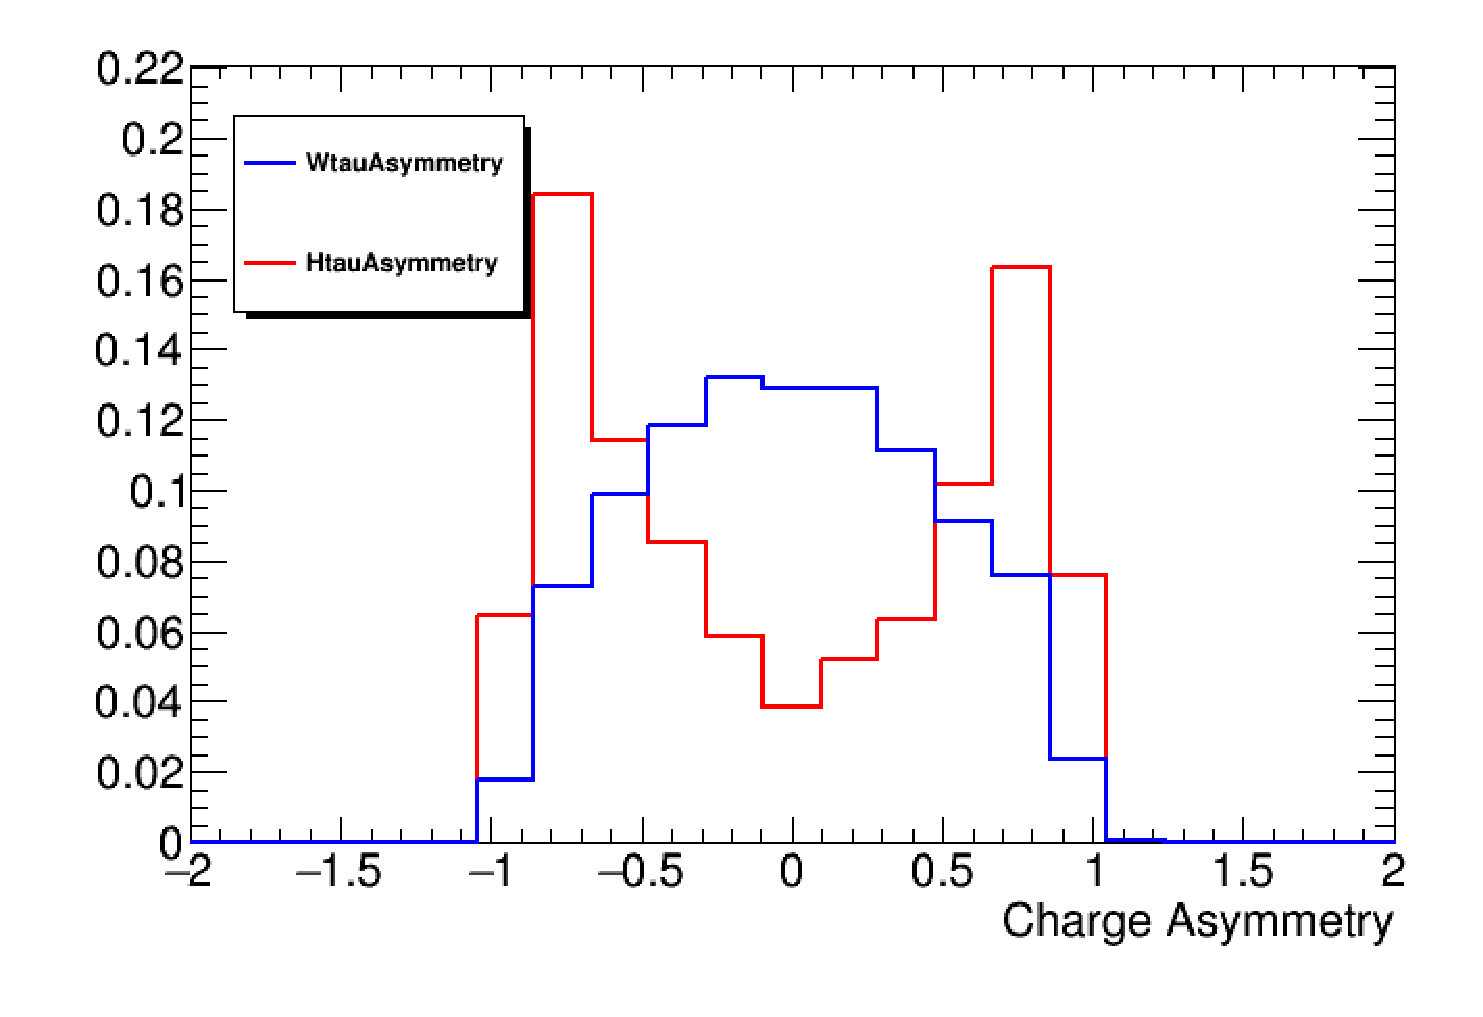
\includegraphics[height=0.32\textwidth]{tauAsy.eps}
\caption{Distribution of tau polarization for Higgs and W decays ;  Postdoc}
\label{fig:tau}
\end{center}
\end{figure}
The tau polarization can be used to separate the W \too $\tau \nu$ background from the signal.  The intrinsic polarization of W$^+$ is -1 while that of $H^+$ is +1.  The tau polarization is defined as $P_{\tau}=\frac{\sigma_R - \sigma_L}{\sigma_R + \sigma_L}$.
A plot of the charge asymmetry, defined as $\Upsilon=\frac{\pt_{track}}{\pt} - 1$, is shown for the signal and background in the $\tau$ \too $\rho \nu_{\tau}$ final in figure~\ref{fig:tau}. Other 1-prong decays will also have similar separation in the charge asymmetry. 
The 1-prong decays can be separated from the 3-prong decays in the final fitting machinery and added statistically together.  This variable will be used as additional variable to the fit in the 1-prong case.

\paragraph{Use matrix element method to reduce true tau background ;  Hadavand, Akafzade}
In addition to the tau polarization one can utilize the event kinematics by utilizing the matrix element method to distinguish the signal from the true tau background originating from \ttbar events.  
By looking at the distribution $d(x)=\frac{P_S(x)}{P_S(x)-P_B(x)}$ where $P_S$ and $P_B$ correspond to the weights from the signal and background 
hypothesis. I have performed initial tests with MadWeight for achieving this goal. This variable can then be added as one of the variables in the BDT. 

\paragraph{Use boosted decision trees ;  Postdoc and Akafzade}
As mentioned earlier for early Run 2 results the discriminating variable used in the fit was $m_T$. As an alternative we can incorporate several 
variables into a bdt and use that output as the discriminating variable in the fit machinery.  Some variables that have been investigated in some preliminary studies
are $m_T$, leading b jet \pt\ , $\tau$ \pt, MET, $\Delta \eta(\tau-$leading jet), $\Delta \phi(top-$sub-leading jet).

\paragraph{Determine jet \too $\tau$ Background from Control Region ;  Hadavand, Akafzade}  %( R2-1, R3-1 - 3 months ) 
For Run 1 the systematics for the $\tau$ \too jet background were one the largest in the analysis.  Due to low statistics at the high mass a fit above 200 GeV was necessary to get 
an estimate of the background in that region.  This is important since this is the dominant background in the high mass region and without a background model the limit machinery would fail.
As an alternative to the matrix method used for the Run 1 published paper one can use a control region with no signal and loosen the selection criteria to introduce more fake taus.  This can be done
by requiring a zero bjet region and only requiring a loose tau selection.  The normalization of this background can then be derived within the fit to data.  This should reduce both the statistical and systematic uncertainty of the analysis.
%In order to attain a control region with enough statistics when imposing this selection criteria one has to change the current trigger which already imposes a selection of a medium tau.  
The use of the tau plus MET trigger has caused some of the main issues with statistics for the QCD background in Run 1. I proposed to use a MET trigger which actually had higher efficiency than the tau plus MET trigger.  
The use of this trigger increases the statistics for the background estimation.
%Other control region which are void of signal can be used in a similar fashion by fitting the normalization within the data.


%\paragraph{Port Statistics Tool to new Naming Convention} ( R2-1 - 2 months )
%The statistics tools written for this analysis by myself and the UTA group have to be changed to accommodate the naming convention imposed by the new xAOD data format.  This will effect the systematic naming only.  It seems 
%like a trivial task but with around 70 nuisance parameters it can be quite tedious to implement.  Mr. Feremenga would benefit from doing this work so as to familiarize himself with the statistics framework of the analysis.

\paragraph{Optimize Binning for Limits ;  Postdoc} %( R2-1 - 2 months )
The low statistics in the tail of the distribution has made the H$^+$ \too $\tau \nu$ channel difficult for setting limits.  In many cases we found that several systematic variations performed for pull determination would make the fits fail.  
This has to do with the fact that the data has low stats and is spiky since similar statistics in smooth MC did not cause the same failures.  By making requirements on signal over background and the number of total background in a given
bin and then testing with pull estimation I was able to optimize the best binning for both stability and sensitivity.  For doing Run 2 projections each luminosity value had to be re-optimized to get the a more realistic projection.
Keeping the binning the same would result in an underestimate of the results. 

\paragraph{Perform Limit Calculations and Fit studies ;  Akafzade}% (R2-1, R3-1 - 1 months)
At this point UTA has quite a bit of experience with the limit setting software. The machinery will be changed with respect to the early Run 2 measurements by adding 
two categories, 1 prong and 3 prong tau decays.  The 1 prong tau decay channel will have an additional variable, the tau polarization variable.  This variable could be adding to the BDT 
but I believe one can gain more by using the shape as a pdf in the fit.
%Mr.  Akafzade should take over this machinery and be able to perform the final limits and also do the fit validation by making pull distributions for all the mass points.

\paragraph{Perform Combination with direct and indirect Searches ;  Postdoc}% (R2-2, R3-1 - 1 months)
For dataset R2-2 and R3-2 where we aim for a publication we can combine the results with direct decays of \Hp and indirectly through the neutral CP odd Higgs decays.  For direct searches we would combine \Hp \too $\tau \nu $ lepton final state where one will
require an additional lepton from the top decay with the hadronic channel.  Combination with the \Hp to tb channel is not required since they cover unique regions in the \tanb\ vs mH plane. This combination will give limits within the \tanb\ and mA plane as well as \tanb\ and cos($\beta-\alpha$) plane. 
One can also combine with indirect searches namely with A \too $\tau \tau$ and A \too Z h final states to make further exclusion over these two planes for various models.

\paragraph{Perform Model Dependent Limits ;  Postdoc} %(R2-2, R3-1 - 1 months)
After branching fraction and cross section limits are performed model dependent limits can be made to determine exclusions of certain models.  Models can include mhmax$\pm$, tauphobic, 2HDM Type III, Type IV, etc.  
%Dr. Montoya has previous experience and software to make these plots.

%\begin{figure}\label{fig:plot1}
%%\begin{center}
%\includegraphics[height=0.32\textwidth]{prospect_mhmodp.eps}
%\includegraphics[height=0.32\textwidth]{prospect_mhmodm.eps}
%\caption{{ 13 TeV projection on limits in the \tanb\ vs M\Hp plane for the MSSM m$_h^{\rm mod}\pm$}}
%\label{fig:lumipros}
%\end{center}
%\end{figure}

\subsubsection{Z+X including Higgs and Taus}
The subsequent sections describe the work needed for the schedule presented on table~\ref{tab:sched}. Each task is listed next to the personnel performing the task.

\paragraph{Determine Algorithm for Boosted/Collimated di-tau Pair Identification ; Postdoc} %(April 2017)
Since we are performing a general search where an unknown particle can decay to a Z boson and another potentially unknown particle, some events will have highly boosted and/`or highly collimated di-tau pairs that regular
tau reconstruction does not treat.  There has been work on ATLAS in this front aimed for reconstructing the channel A \too Z(ll) h($\tau\tau$)~\cite{di-tau-thesis}.  In this case the \pt of the di-tau system is quite high of an order of 500 GeV.
In other cases the \pt of the di-tau system can be small but they can be highly collimated.  This has been seen in the h \too a($\mu \mu$) a($\tau \tau$) analysis.  In fact the algorithm developed for A \too Z(ll) h($\tau\tau$) would not 
work for this channel because of the large \pt cut and the fact that it is seeded by a large R (1.0) Jet.  Large R jets only have calibration available for \pt larger than 200 GeV.  So I propose to develop a high \pt di-tau
algorithm and a low \pt highly collimated algorithm where standard jets of R of 0.4 can be used. A boosted decision tree (BDT) can be developed using the jet substructure information.  
The variables suggested to be used in the BDT are as follows:
\begin{itemize}
\item{core energy fractions, $f_{core}^{sub(lead)}=\frac{\sum_{cells}^{\Delta R=0.1} \pt_{cell}}{\sum_{cells}^{\Delta R=0.2}\pt_{cell}} $}
\item {The subjet energy fractions $f(sub)lead_{subjet}=\frac{\pt^{subjet}}{\pt^{Jet}}$. }
\item{leading track momentum fractions $f(sub)lead_{subjet}=\frac{\pt ^{leadTrack}}{\pt^{subjet}}$}
\item{the maximum track distance Rmax}
\item{the number of tracks n(sub)leading track.}
\end{itemize}

\paragraph{Write General Analysis Suite for xAODs;  Postdoc, Akafzade} %(April 2017)
%The postdoc I will design and develop an analysis suite for the Z scan analysis.  
This analysis has leptons including taus in the final states so the analysis suite can be generalized but always adding a constraint of having a Z boson in the final state. 
 %The Z(dark)Z(dark) channel including four electrons will be left out of the analysis here due to the many channels already being explored.  This is to ensure
%symmetry between the h \too aa and Z(dark)Z(dark) making it easily combined in one analysis.  
Since we would like to perform an inclusive search of any particle decaying to Z+X we will keep this analysis suite very general. 
However, on top of the general analysis suite one can build tools to make additional requirements on the specific states. For example if there is mass constraint that can be imposed such as the mass of the Higgs.
%For example for the muon scan we can require that the two particle masses are within some limit of each other ie $\cbar$m(a$_1$)-m(a$_2$)\cbar$< \epsilon$ where $\epsilon$ will be governed by the detector resolution 
%of the different objects or just the natural width of the particle.  The resolution will matter for different pt objects or whether looking at the tau or muon final states.

\paragraph{Determine Background Parameterization from Control Regions, $\mu\mu$ scan ;  Postdoc, Akafzade, Hadavand}
Two control regions (CRs) are used in this analysis to constrain the SM backgrounds in the final fit to the data. The first region, CRj, is used to constrain the 
low mass SM resonances and Drell-Yan dominated non-resonant background. The second region, CRb, is used to constrain the \ttbar\ non-resonant background.
Both regions are defined by first requiring a tagged $\mu\mu$ candidate. CRj is further required to have
at least one selected jet and not be b-tagged. CRb is required to have at least two selected jets that have been b-tagged.
Any events which are in one of the SRs are excluded from the two CRs.

\paragraph{Determine Background Parameterization from Control Regions, $\tau\tau$ scan ;  Postdoc, Akafzade, Hadavand}
The control region used to determine the parametrization of the jets faking tau objects is defined as having two same sign tau leptons and inverting one of the tau identification criteria.
Simulation is used to predict the shape of the contribution from events with two true leptons and hadronically-decaying tau that are either correctly reconstructed or reconstructed
from leptons or leptonically-decaying taus.  These two parameterizations of the two backgrounds is then used to fit to the data as a more sophisticated template method.  The sidebands of the Z boson
can be used to validated this approach.

\paragraph{Parameterize Background ;  Akafzade, Hadavand} %(D - 3 months) 
As described in section~\ref{sec:zscanback} the backgrounds to the multiple BSM analysis  will be J/$\psi$, $\upsilon$, \ttbar, Drell-Yan, and Z tails.  One can 
parameterize these background from the control regions described above then fit for the normalization within the signal region similar to what is done in the
$\tau\tau \mu \mu$ analysis on ATLAS~\cite{tautaumumu}.  We also have the SM ZZ* as a non-peaking background which may be difficult to model. This background and the SM resonant backgrounds 
can be parameterized with MC and used in the fits. I have extensive experience with parameterized fits from the \babar\ experiment and can guide my graduate student to model the various SM backgrounds.

\paragraph{Perform two separate scans in Z final state ;  Postdoc, Akafzade} %(D - 4 months)
In the decay of Y \too Z + X we call the mass of X can be reconstructed as X(ee), X($\mu\mu$), and X($\tau\tau$).  
The three Z scans look at the X(ee),X($\mu\mu$), and X($\tau\tau$) mass spectrum. For the X(ll), l=e,$\mu$ spectrum the Z will be reconstructed as Z($\tau\tau$).  For the X($\tau\tau$) spectrum the Z will be reconstructed in Z(ll), l=e,$\mu$.  
%By adding the various Z final states to the same spectrum we increase the statistics which will make it easier for the bump-hunter to determine if there is a signal.
The X(ee) and X($\mu\mu$) can be potentially combined if the resolution of the particles are similar enough.  The X($\tau\tau$) will not be combined with X(ll) l=e,mu since the resolution is quite different and the bump-hunter would not gain in looking for two overlapping bumps of vastly differing resolutions.
The use of the bump-hunter will allow for a first statistical pass at the data to determine if there is an existence of signal in the samples.  


%\paragraph{Muon Scan - aa and Z(dark)Z(dark) final state scan} (D - 4 months)
% The muon scan will look only at the m($\mu\mu$) and combine five final states in one mass spectrum.  The five final states include a($\mu\mu$)+$\Bigg(${a($\mu\mu$),a($\tau\tau$), Z(dark)($\mu\mu$), Z(dark)(ee), and Z(dark)($\tau\tau$)$\Bigg)$. The four electron final state will not be reconstructed for Z(dark)Z(dark) in this manner so to make the
% the analysis more simplified given the ambitious number of
% channels we aim to analyze in each scan.  The dilepton pair that are not scanned, 'other', will be reconstructed in m$_{\rm other}$(ll) l=e,$\mu$, $\tau$. The combination of these three channels will be combined to look at the dimuon mass spectrum.  A clear peak should appear in the presence of the narrow resonances
% of the scalar a and Z(dark).  My graduate student should be able to run the analysis suite and make these distributions.

%\paragraph{Determine other Discriminating Variables} (D - 4 months) 
%For the $\tau\tau$ final states an MMC calculator should be used for the Z scan analysis.  One can investigate the use of the Higgs mass to make peaks sharper.  For the $\mu$ scan can
%since the decay is to two identical particles can use an additional constraint on the mass in that way.  In doing so one much be careful in comparing masses of two taus to two leptons since the tau resolution will be a bit factor in the matching.  
%This is work that my graduate student can perform.

\paragraph{Develop and Optimize Bump-hunter to Scan Data ;  Hadavand, Akafzade} %(April '17)
I have previously worked on a bump-hunter which would be independent of the signal model used.  I called this program Signal Parameter Independent Fit (SPIF).  Using the parametrization described above we fit the data and remove a window where signal is expected.
The background is then extrapolated within this window and the difference of the number of events in the window versus the fit extrapolation is determined.  A p-value is determined using Poisson statistics for the difference between the number of events in the window and the extrapolated background within the window.
A scan is done using as input the step size and a of range of window sizes.  Several scans are performed changing the window size and step size iteratively until the p-value no longer improves within a specified precision.  
Once all iterations are performed, the window(s) with the smallest p-value(s) is(are) reported.  
%Using the bump-hunter can also work for blind analysis where only information about the significance of a  bump is presented but the total distribution can remain blind.
%Doing a bump-hunter scan can also save time in determining limits since putting limits on the entire distribution in very fine binning will take lots of CPU power.  
If the bump-hunter analysis reports no significant signal then a coarser binning can be used for the limit setting saving time and CPU power.



\paragraph{Perform validation of bump-hunting technique ;  Akafzade} %(D - 2 months) 
To validate the performance of the bump-hunter in a specific environment one should test by injecting signal over the analytically determined background to see if the fit poses any biases and to test the sensitivity of the method in the presence of
a specific type of signal as determined by various signal MC.  The iterative method used to hone in on the signal can be tested in to ensure no biases are present.

%\paragraph{Use tau handedness to Separate Z and Higgs decays} (now-Feb 2015)
%When performing the Z mass scan and it is determined that the SM h \too ZZ* is a large background to the A \too Z h final state we can perform a helicity cut to remove the Z* decays leaving in the scan only the resonant 
%decays.  This would only appear in the m($\tau\tau$) distribution where the Z would be reconstructed in the Z(ll) final states.  This will also make the work of the bump-hunter in this channel much easier since a broad shoulder 
%will be difficult to distinguish with a bump-hunter unless it is alternatively fitted out as a background.


%\paragraph{Optimize Binning for Limits } %(D - 2 months)
%Since in many cases we are looking in masses as high as a few TeV the background statistics will be limited in that region.  It is therefore important to perform binning optimization as it has been done 
%for the \Hp analysis to ensure the stability of the fit and to achieve the best possible limits in the absence of signal. The binning optimization is done by choosing different values of signal over background and total number of background to ensure the stability of the fits yet
%allow for the best possible limits.  This work can be done by myself and soon taken over by my graduate student.

\paragraph{Develop Limit setting software for various final states ;  Akafzade, Postdoc} %(D - 2 months)
%My extensive experience in developing limits setting software within the RooFit and RooStats framework will make this task somewhat simple to have my graduate student perform.  The most tedious part will be dealing systematics which will be in common across all the channels so time is saved in having 
%originally harmonized analysis.  This is work that I can initiate with the help of Mr. Akafzade.
Once the background is parameterized and the normalization is determined from the signal region, we can determine limits using a binned maximum likelihood fit using  HistFactory as is usually done on ATLAS. 
For a search in a large window of mass typically a fine grid of masses are tested.  However with the input from the SPIF program we can only use a fine grid in regions where the p0 value is low indicating some deviation
from the background.  This will save CPU time in setting the final limits. 
Since our search includes several final states, these final states must be statically combined for each channel to get the best limits. 

\paragraph{Perform Model Dependent Exclusions ;  Postdoc} %(D - 1 months)
With the use of the branching fractions for each model exclusions on various model parameters can be made using the cross section limits. For NMMSM or 2HDM the exclusions will be in the \tanb\ vs mA plane and \tanb\ vs $\cos(\beta-\alpha)$ plane.
\subsubsection{Tile HL-LHC LVPS Upgrade}
The preliminary schedule and tasks for the Tile HL-LHC LVPS upgrade project is shown in table~\ref{tab:lvps}.
%The production of bricks will end by 2022 but only the timeline relevant to this proposal has been shown.
\begin{table}[htb]
\begin{center}
\begin{tabular}{       l  |l |l | l                } \\ 
\rowgroup{\textbf{Task} }& \textbf{Personnel} &\textbf{Start Date} & \textbf{End Date}   \\ \hline\hline
\rowgroup{\textbf{New Burn-in Station Design and Fabrication}}   & Hibbard, EA, EE&  01/30/17   &  12/15/17  \\ \hline  
\rowgroup{\textbf{Prototype}}                                   &  - &01/29/18    & 08/30/19 \\ \hline
Procurement of brick components for prototype V8.2 bricks   &  Hibbard, EA &01/29/18 & 05/11/18  \\ 
Basic Check-out and burn-in (Prototype) & Hibbard, EA &  04/22/19   &  05/24/19 \\  
Prototype Review   & EE, EA & 05/27/19   &  08/30/19   \\
Integration and testing of vertical slice   &  Hibbard, EA &06/03/19   &  07/26/19  \\ \hline
\rowgroup{\textbf{Finalize  V8.3 pre-production design} }  & EA, EE & 07/29/19  & 08/23/19 \\ \hline
\rowgroup{\textbf{LVPS pre-production design review}}   &  EA, EE & 08/26/19   &  08/30/19 \\  \hline 
\rowgroup{\textbf{Pre-production}}   & - & 09/2/19    & 12/30/20   \\ \hline 
  Check-out and burn-in tests on pre-production bricks & EA, undergrads  &  07/06/20   &  09/25/20 \\ 
  Ship bricks to CERN   & EA & 09/28/20 & 10/02/20  \\
  Integration tests at CERN and final review   & EA & 10/05/20   &  12/31/20 \\ \hline
\rowgroup\textbf{{Production}  } &  - & 01/04/21 &   04/08/22  \\ \hline

  Production PCB Assembly   &  EE,EA & 04/12/21   &  06/04/21  \\ 
  Check-out and burn-in (16 to start and find any issues)  & undergrads   &   04/19/21   &  04/30/21 \\  
  Check-out and burn-in (64 to confirm production) & undergrads  &  05/03/21   &  05/28/21 \\  
  Check-out and burn-in (1000)   & undergrads  & 05/31/21   &  04/08/22  \\  \hline
\end{tabular}
\caption{ The HL-LHC Tile LVPS upgrade schedule.}
\label{tab:lvps}
\end{center}
\end{table}




\begin{thebibliography}{99}

\bibitem{atlhi} {} ATLAS Collaboration, Observation of a new particle in the search for the Standard Model
Higgs boson with the ATLAS detector at the LHC, Phys. Lett. B 716 (2012) 1-29,
[arXiv:1207.7214].
 \bibitem{cmshi} {} CMS Collaboration, Observation of a new boson at a mass of 125 GeV with the CMS
experiment at the LHC, Phys. Lett. B 716 (2012) 30-61, [arXiv:1207.7235].
\bibitem{atlbo} {} ATLAS Collaboration, Measurements of Higgs boson production and couplings in diboson
final states with the ATLAS detector at the LHC, Phys. Lett. B 726 (2013) 88-119,
[arXiv:1307.1427].
\bibitem{atlsp} {}  ATLAS Collaboration, Evidence for the spin-0 nature of the Higgs boson using ATLAS data,
Phys. Lett. B 726 (2013) 120-144, [arXiv:1307.1432].
\bibitem{cmsf} {} CMS Collaboration, Evidence for the direct decay of the 125 GeV Higgs boson to fermions,
Nature Phys. 10 (2014) [arXiv:1401.6527].
\bibitem{cmsbo} {}  CMS Collaboration, Measurement of the properties of a Higgs boson in the four-lepton final
state, Phys.Rev. D 89 (2014) 092007, [arXiv:1312.5353].
\bibitem{cmspro} {}  CMS Collaboration, Measurement of Higgs boson production and properties in the WW decay
channel with leptonic final states, JHEP 01 (2014) 096, [arXiv:1312.1129].
\bibitem{eng}{} F. Englert and R. Brout, Broken symmetry and the mass of gauge vector mesons,
Phys. Rev. Lett. 13 (1964) 321–323.
\bibitem{higgs1}{} P. W. Higgs, Broken symmetries, massless particles and gauge fields, Phys. Lett. 12 (1964)
132–133.
\bibitem{higgs2}{} P. W. Higgs, Broken symmetries and the masses of gauge bosons, Phys. Rev. Lett. 13 (1964)
508–509.
\bibitem{higgs3}{} P. W. Higgs, Spontaneous symmetry breakdown without massless bosons, Phys. Rev. 145
(1966) 1156–1163.
\bibitem{intermediate}{} Intermediate Mass calculations, to appear in arxiv.

\bibitem{women}{} Marie-Claire Shanahan, "Can we declare victory for women in their participation in science? Not yet", Scientific American Blog, March 29, 2011.
\bibitem{women1}{} Rachel Ivie, Susan White, Arnell Garrett, and Garrett Anderson, "Women among Physics and Astronomy Faculty Results from the 2010 Survey of Physics Degree-Granting Departments", 
https://www.aip.org/statistics/reports/women-among-physics-astronomy-faculty, August, 2013.
\bibitem{women3}{} P. Gaganon, "Women in physics: Are we there yet?", Quantum Diaries, http://www.quantumdiaries.org/2012/10/31/women-in-physics-are-we-there-yet/
\bibitem{bab0} {}B.~Aubert {\it et al.}  [BABAR Collaboration], ``Measurement of the \Bu/\Bz production ratio from the \FourS meson using \Bp $\to$ \jpsi \Kp and \Bz $\to$ \jpsi \KS decays'', {}Phys.\ Rev.\ D {\bf 69}, 071101 (2004).
``New Physics results from the \babar\ Collaboration'', July 2005.
\bibitem{bab1} {}B.~Aubert {\it et al.}  [BABAR Collaboration],
``Branching Fraction and \CP Asymmetries in \Bz $\to$ \KS \KS \KS'',
  Phys.\ Rev.\ Lett.\  {\bf 95}, 011801 (2005).
\bibitem{atl5b}
  S.~Kolos, A.~Corso-Radu, H.~Hadavand, M.~Hauschild, R.~Kehoe,
  ``A software framework for Data Quality Monitoring in ATLAS'',
  J.\ Phys.\ Conf.\ Ser.\  {\bf 119}, 022033 (2008).
\bibitem{atl6}  {}Peter Renkel, Haleh Hadavand, Robert Kehoe, ``The Gatherer - a mechanism for integration of monitoring data in ATLAS'', {}, J.\ Phys.\ Conf.\ Ser.\  {\bf 219}, 022043 (2010).
\bibitem{atl2} {} The ATLAS Collaboration, ``Search for Diphoton Events with Large Missing Transverse Energy in 7 TeV Proton-Proton Collisions with the ATLAS Detector'', Phys.\ Rev.\ Lett.\  {\bf 106}, 121803 (2011).
\bibitem{atl1} {} The ATLAS Collaboration, ``Search for extra dimensions using diphoton events in 7 TeV proton-proton collisions with the ATLAS detector", Phys.\ Lett.\ B {\bf 710}, 538-556 (2012).
\bibitem{atl1-conf} {} The ATLAS Collaboration, ``A Search for High Mass Diphoton Resonances in the Context of the Randall-Sundrum Model in $\sqrt s=7$ TeV pp Collisions", ATLAS-CONF-2011-044 (2011).
\bibitem{hptnu} {} The ATLAS Collaboration, "Search for charged Higgs bosons decaying via $H^{\pm} \rightarrow \tau^{\pm}\nu$ in fully hadronic final states using pp collision data at $\sqrt{s}$ = 8 TeV with the ATLAS detector'', ATLAS-CONF-2014-050 (2014).
\bibitem{atl2014} {} The ATLAS Collaboration, "Search for charged Higgs bosons decaying via $H^{\pm} \rightarrow \tau^{\pm}\nu$ in fully hadronic final states using pp collision data at $\sqrt{s}$ = 8 TeV with the ATLAS detector'', JHEP03 (2015) 088.
\bibitem{taunu} {} ATLAS Collaboration, "Search for charged Higgs bosons produced in association with a top quark and decaying via $H^{\pm} \rightarrow \tau^{\pm}\nu$ 
using pp collision data recorded at $\sqrt s$=13 TeV by the ATLAS detector", Phys. Lett. B 759 (2016) 555-574,[arXiv:1603.09203].

\bibitem{hptnu1} {} The ATLAS Collaboration, "Search for charged Higgs bosons decaying via $H^{\pm} \rightarrow \tau^{\pm}\nu$ in fully hadronic final states using pp collision data at $\sqrt{s}$ = 13 TeV with the ATLAS detector'', ICHEP 2016 CONF note (2016).
\bibitem{3lep} {} The ATLAS Collaboration, "Another Search for strongly produced supersymmetric particles in
final states containing a same-flavour opposite-sign dilepton pair, jets and missing transverse momentum in 13 TeV p p collisions", ATL-COM-PHYS-2016-504, 2016.
%\bibitem{susy1}{} P. Fayet, Supersymmetry and Weak, Electromagnetic and Strong Interactions, Phys. Lett.
%B 64 (1976) 159.
%\bibitem{susy2}{} S. Dimopoulos and H. Georgi, Softly Broken Supersymmetry and SU(5), Nucl. Phys. B 193
%(1981) 150.

\bibitem{combin}{} ATLAS Experiment, Measurements of the Higgs boson production and decay rates and
coupling strengths using pp collision data at $\sqrt{s}$ = 7 and 8 TeV in the ATLAS experiment, ATLAS-CONF-2015-007.

\bibitem{exohiggs}{} D. Curtin, R. Essig, S. Gori, P. Jaiswal, A. Katz, et al., Exotic Decays of the 125 GeV Higgs Boson,
810 arXiv:1312.4992 [hep-ph],
Phys. Rev. D 85, (2012) 115019.

\bibitem{2hdm1}{} J. F. Gunion, H. E. Haber, G. L. Kane and S. Dawson, Front. Phys. 80, 1 (2000); J. F. Gunion,
H. E. Haber, G. L. Kane and S. Dawson, hep-ph/9302272.
\bibitem{2hdm2}{} G. C. Branco et al, Phys. Rept. 516, 1 (2012) [arXiv:1106.0034 [hep-ph]].
\bibitem{2hdm3}{} J. F. Gunion and H. E. Haber, Phys. Rev. D 67, 075019 (2003) [hep-ph/0207010].
\bibitem{zdark}{} Hooman Davoudiasl, Hye-Sung Lee, and William J. Marciano, “Dark” Z implications for parity violation, rare meson decays, and Higgs physics
%\bibitem{hexotic}{} D. Curtin, R. Essig, S. Gori, P. Jaiswal, A. Katz, et al., Exotic Decays of the 125 GeV Higgs Boson, arXiv:1312.4992 [hep-ph].
\bibitem{2016:4l}{} ATLAS Collaboration, "Event selection and background estimation in the H \too ZZ$^*$ \too 4l channel at $\sqrt x=13$ TeV - ICHEP 2016 Analysis", ATL-COM-PHYS-2016-413, 2016.

\bibitem{di-tau-thesis}{} D.Kirchmeier, "Reconstruction and Identification of Boosted Tau Pair Topologies at ATLAS", ATLAS Thesis, CERN-THESIS-2015-220.
\bibitem{tautaumumu}{} A. Haas and B. Kaplan, Search for h \too aa decays in the NMSSM in the $\mu\mu\tau\tau$ channel using 20.3/fb of pp collisions at $\sqrt{s}$ = 8 TeV using the ATLAS detector, ATL-COM-PHYS-2014-278.  
\end{thebibliography}
\end{document}
